\documentclass[aspectratio=169]{beamer}

\usetheme{default}
\usecolortheme{dove}

\setbeamertemplate{navigation symbols}{}
\setbeamertemplate{footline}{%
  \hfill{\large\insertframenumber\,/\,\inserttotalframenumber}\hspace{0.8em}\vspace{0.5em}%
}

\definecolor{popblue}{RGB}{52, 101, 164}
\definecolor{sampred}{RGB}{204, 0, 0}
\definecolor{paramgreen}{RGB}{0, 140, 70}
\definecolor{warnred}{RGB}{180, 40, 40}
\definecolor{orange1}{RGB}{220, 120, 0}
\definecolor{violet1}{RGB}{120, 50, 160}
\definecolor{lightbg}{RGB}{245, 245, 250}

\setbeamercolor{frametitle}{fg=popblue}
\setbeamercolor{title}{fg=popblue}

\usepackage{pgfplots}
\usepackage{tikz}
\usetikzlibrary{shapes, arrows.meta, positioning, calc, decorations.pathreplacing, patterns}
\pgfplotsset{compat=1.18}
\usepackage{amsmath, amssymb}
\usepackage{pifont}
\usepackage{fontenc}

\title{Lecture 9: Hypothesis Testing}
\subtitle{p-Values $\cdot$ Power Analysis $\cdot$ Permutation Tests $\cdot$ Multiple Testing}
\date{}

\begin{document}

% ============================================================
\begin{frame}
\titlepage
\end{frame}

% ============================================================
\begin{frame}
\frametitle{Previously, on Lecture 8\ldots}

\begin{center}
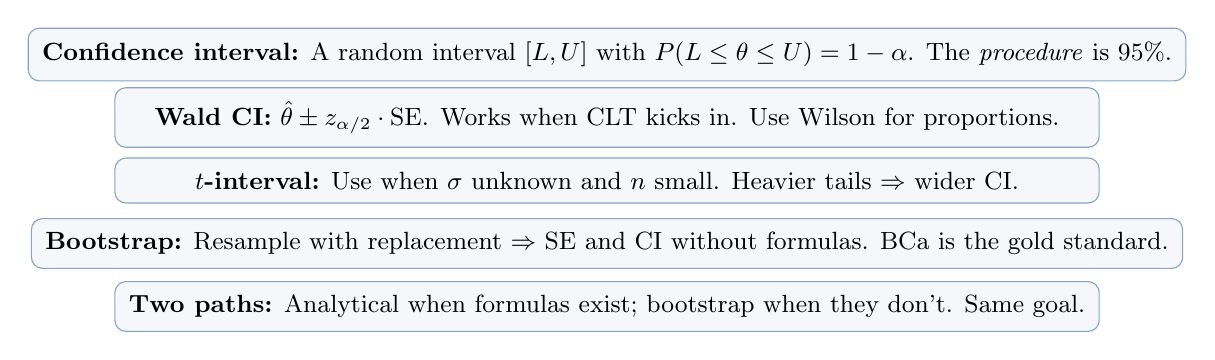
\begin{tikzpicture}[
  sbox/.style={draw=popblue!60, fill=popblue!5, rounded corners=4pt, minimum width=12.5cm, minimum height=0.5cm, align=left, inner sep=5pt, font=\small}
]
  \node[sbox] at (0, 2.0) {\textbf{Confidence interval:} A random interval $[L, U]$ with $P(L \leq \theta \leq U) = 1 - \alpha$. The \textit{procedure} is 95\%.};
  \node[sbox] at (0, 1.2) {\textbf{Wald CI:} $\hat\theta \pm z_{\alpha/2} \cdot \text{SE}$. Works when CLT kicks in. Use Wilson for proportions.};
  \node[sbox] at (0, 0.4) {\textbf{$t$-interval:} Use when $\sigma$ unknown and $n$ small. Heavier tails $\Rightarrow$ wider CI.};
  \node[sbox] at (0, -0.4) {\textbf{Bootstrap:} Resample with replacement $\Rightarrow$ SE and CI without formulas. BCa is the gold standard.};
  \node[sbox] at (0, -1.2) {\textbf{Two paths:} Analytical when formulas exist; bootstrap when they don't. Same goal.};
\end{tikzpicture}
\end{center}

\vspace{0.3cm}
\begin{center}
{\large\textbf{Today:}} We can estimate and quantify uncertainty. Now: is the effect \textbf{real} or \textbf{noise}?
\end{center}
\end{frame}

% ============================================================
% PART I: THE LOGIC OF TESTING
% ============================================================
\section{The Logic of Testing}

\begin{frame}
\begin{center}
  \vspace{1.5cm}
  {\Huge\bfseries\textcolor{popblue}{Part I: The Logic of Testing}}

  \vspace{0.8cm}
  {\large Is 3\,mmHg a real effect or just noise?}
\end{center}
\end{frame}

\begin{frame}
\frametitle{The Drug Trial}

\begin{center}
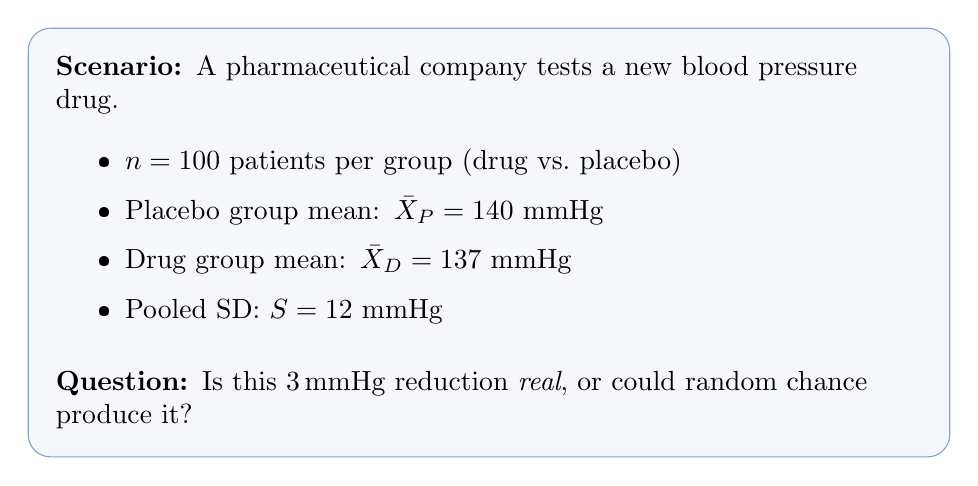
\begin{tikzpicture}
  \node[draw=popblue!60, fill=popblue!5, rounded corners=8pt, text width=11cm, align=left, inner sep=10pt] {
    \textbf{Scenario:} A pharmaceutical company tests a new blood pressure drug.\\[4pt]
    \begin{itemize}\setlength{\itemsep}{2pt}
      \item $n = 100$ patients per group (drug vs.\ placebo)
      \item Placebo group mean: $\bar{X}_P = 140$ mmHg
      \item Drug group mean: $\bar{X}_D = 137$ mmHg
      \item Pooled SD: $S = 12$ mmHg
    \end{itemize}
    \vspace{4pt}
    \textbf{Question:} Is this 3\,mmHg reduction \textit{real}, or could random chance produce it?
  };
\end{tikzpicture}
\end{center}

\vspace{0.2cm}
\begin{center}
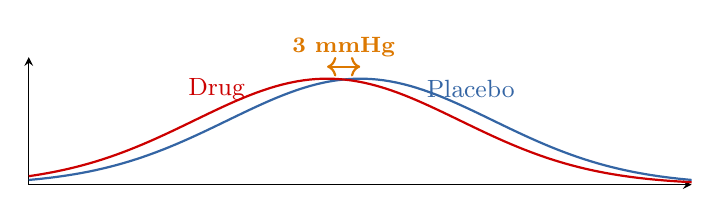
\begin{tikzpicture}
  % Two overlapping Normal curves
  \begin{axis}[
    width=10cm, height=3.2cm,
    domain=110:170, samples=100,
    axis lines=middle, ticks=none,
    ymin=0, ymax=0.04,
    xmin=110, xmax=170,
    every axis plot/.style={thick, no markers},
    clip=false
  ]
    \addplot[popblue, thick] {exp(-0.5*((x-140)/12)^2) / (12*sqrt(2*pi))};
    \addplot[sampred, thick] {exp(-0.5*((x-137)/12)^2) / (12*sqrt(2*pi))};
    \draw[<->, thick, orange1] (axis cs:137, 0.037) -- (axis cs:140, 0.037)
      node[midway, above, font=\footnotesize\bfseries] {3 mmHg};
    \node[font=\small, popblue] at (axis cs:150, 0.03) {Placebo};
    \node[font=\small, sampred] at (axis cs:127, 0.03) {Drug};
  \end{axis}
\end{tikzpicture}
\end{center}
\end{frame}

\begin{frame}
\frametitle{Innocent Until Proven Guilty}

\begin{center}
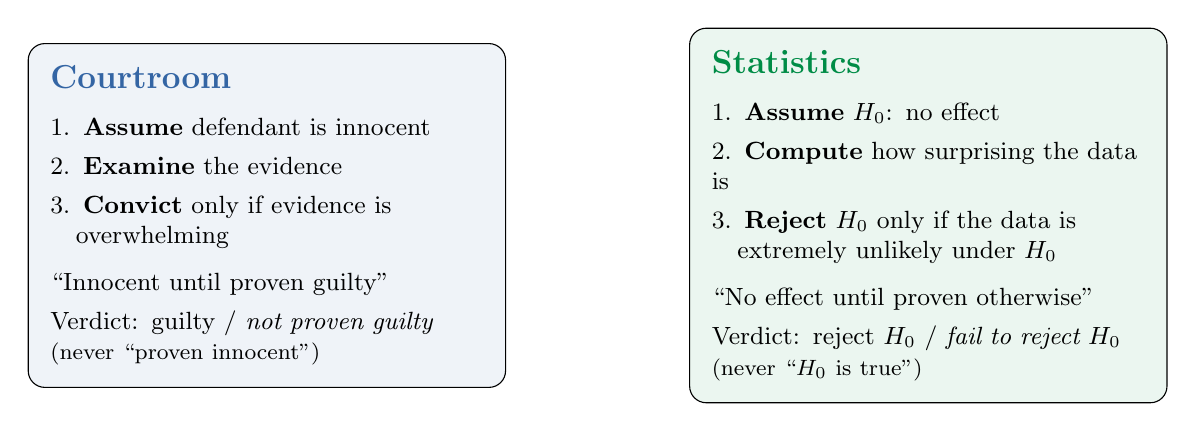
\begin{tikzpicture}[
  cbox/.style={draw, rounded corners=6pt, minimum height=4.2cm, text width=5.5cm, align=left, inner sep=8pt, font=\small}
]
  \node[cbox, fill=popblue!8] at (-4.2, 0) {
    \textbf{\large\textcolor{popblue}{Courtroom}}\\[6pt]
    1. \textbf{Assume} defendant is innocent\\[3pt]
    2. \textbf{Examine} the evidence\\[3pt]
    3. \textbf{Convict} only if evidence is\\
    \quad overwhelming\\[6pt]
    ``Innocent until proven guilty''\\[3pt]
    Verdict: guilty / \textit{not proven guilty}\\
    \footnotesize (never ``proven innocent'')
  };

  \node[cbox, fill=paramgreen!8] at (4.2, 0) {
    \textbf{\large\textcolor{paramgreen}{Statistics}}\\[6pt]
    1. \textbf{Assume} $H_0$: no effect\\[3pt]
    2. \textbf{Compute} how surprising the data is\\[3pt]
    3. \textbf{Reject} $H_0$ only if the data is\\
    \quad extremely unlikely under $H_0$\\[6pt]
    ``No effect until proven otherwise''\\[3pt]
    Verdict: reject $H_0$ / \textit{fail to reject $H_0$}\\
    \footnotesize (never ``$H_0$ is true'')
  };
\end{tikzpicture}
\end{center}
\end{frame}

\begin{frame}
\frametitle{$H_0$ and $H_1$}

\begin{center}
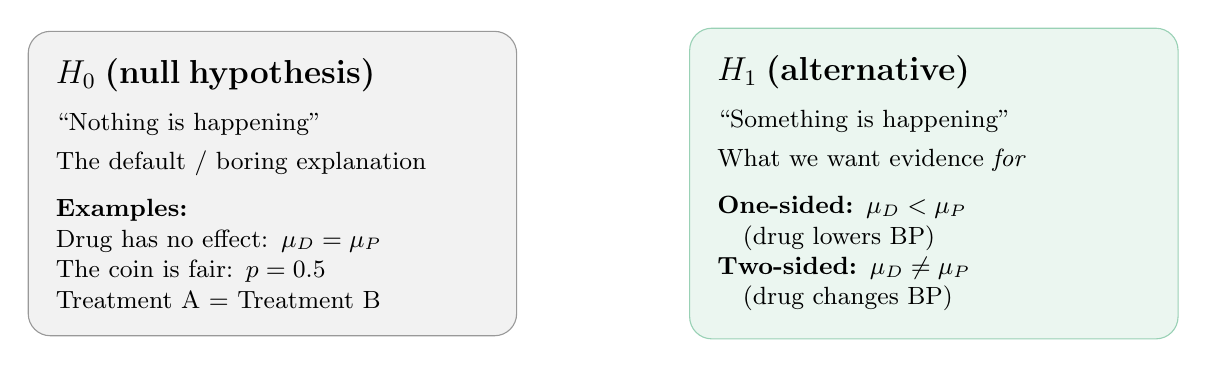
\begin{tikzpicture}[
  hbox/.style={draw, rounded corners=8pt, text width=5.5cm, align=left, inner sep=10pt, font=\small, minimum height=2.8cm}
]
  \node[hbox, fill=black!5, draw=black!40] at (-4.2, 0.5) {
    {\large\textbf{$H_0$ (null hypothesis)}}\\[6pt]
    ``Nothing is happening''\\[3pt]
    The default / boring explanation\\[6pt]
    \textbf{Examples:}\\
    Drug has no effect: $\mu_D = \mu_P$\\
    The coin is fair: $p = 0.5$\\
    Treatment A = Treatment B
  };

  \node[hbox, fill=paramgreen!8, draw=paramgreen!40] at (4.2, 0.5) {
    {\large\textbf{$H_1$ (alternative)}}\\[6pt]
    ``Something is happening''\\[3pt]
    What we want evidence \textit{for}\\[6pt]
    \textbf{One-sided:} $\mu_D < \mu_P$\\
    \quad (drug lowers BP)\\
    \textbf{Two-sided:} $\mu_D \neq \mu_P$\\
    \quad (drug changes BP)
  };
\end{tikzpicture}
\end{center}

\vspace{0.1cm}
\begin{center}
\fcolorbox{orange1}{orange1!5}{\parbox{11cm}{\centering\small
  \textbf{Key:} We never ``prove'' $H_0$. We either \textbf{reject} it (strong evidence against)\\
  or \textbf{fail to reject} it (insufficient evidence). Absence of evidence $\neq$ evidence of absence.
}}
\end{center}
\end{frame}

\begin{frame}
\frametitle{The Test Statistic}

\small
A \textbf{test statistic} $T$ compresses the data into one number measuring ``distance from $H_0$''.

\vspace{0.1cm}
\begin{center}
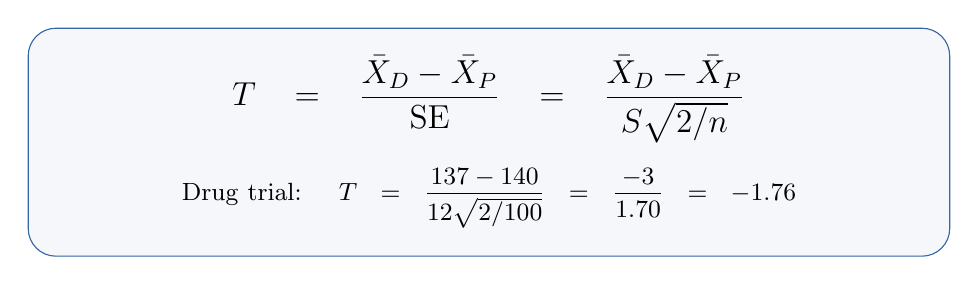
\begin{tikzpicture}
  \node[draw=popblue, fill=popblue!5, rounded corners=10pt, text width=11cm, align=center, inner sep=10pt] {
    {\large $T = \dfrac{\bar{X}_D - \bar{X}_P}{\text{SE}} = \dfrac{\bar{X}_D - \bar{X}_P}{S\sqrt{2/n}}$}\\[8pt]
    \small Drug trial: $\;T = \dfrac{137 - 140}{12\sqrt{2/100}} = \dfrac{-3}{1.70} = -1.76$
  };
\end{tikzpicture}
\end{center}

\vspace{0.1cm}
Under $H_0$: $T \sim N(0, 1)$ approximately. Large $|T|$ = data far from $H_0$ = evidence against $H_0$.

\vspace{0.1cm}
\begin{center}
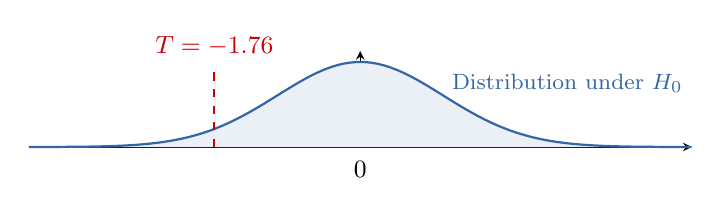
\begin{tikzpicture}
  \begin{axis}[
    width=10cm, height=2.8cm,
    domain=-4:4, samples=100,
    axis lines=middle, ticks=none,
    ymin=0, ymax=0.45,
    every axis plot/.style={thick, no markers},
    clip=false
  ]
    \addplot[popblue!30, fill=popblue!10, draw=none, domain=-4:4] {exp(-0.5*x^2)/sqrt(2*pi)} \closedcycle;
    \addplot[popblue, thick] {exp(-0.5*x^2)/sqrt(2*pi)};
    \draw[thick, dashed, sampred] (axis cs:-1.76, 0) -- (axis cs:-1.76, 0.38);
    \node[font=\small\bfseries, sampred, above] at (axis cs:-1.76, 0.38) {$T = -1.76$};
    \node[font=\small, below] at (axis cs:0, -0.02) {$0$};
    \node[font=\footnotesize, popblue] at (axis cs:2.5, 0.3) {Distribution under $H_0$};
  \end{axis}
\end{tikzpicture}
\end{center}
\end{frame}

\begin{frame}
\frametitle{The Rejection Region}

\small
Choose a \textbf{significance level} $\alpha$ (typically 0.05) \textit{before} looking at the data.

\vspace{0.15cm}
\begin{center}
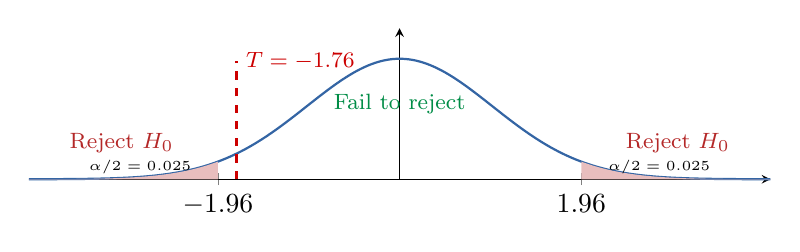
\begin{tikzpicture}
  \begin{axis}[
    width=11cm, height=3.5cm,
    domain=-4:4, samples=200,
    axis lines=middle,
    xtick={-1.96, 0, 1.96},
    xticklabels={$-1.96$, $0$, $1.96$},
    ytick=\empty,
    ymin=0, ymax=0.5,
    every axis plot/.style={thick, no markers},
    clip=false
  ]
    % Main curve
    \addplot[popblue, thick] {exp(-0.5*x^2)/sqrt(2*pi)};
    % Left rejection region
    \addplot[fill=warnred!30, draw=none, domain=-4:-1.96] {exp(-0.5*x^2)/sqrt(2*pi)} \closedcycle;
    % Right rejection region
    \addplot[fill=warnred!30, draw=none, domain=1.96:4] {exp(-0.5*x^2)/sqrt(2*pi)} \closedcycle;
    % Observed T
    \draw[thick, dashed, sampred] (axis cs:-1.76, 0) -- (axis cs:-1.76, 0.39);
    \node[font=\footnotesize\bfseries, sampred, right] at (axis cs:-1.76, 0.39) {$T = -1.76$};
    % Labels
    \node[font=\footnotesize, warnred] at (axis cs:-3, 0.12) {Reject $H_0$};
    \node[font=\footnotesize, warnred] at (axis cs:3, 0.12) {Reject $H_0$};
    \node[font=\footnotesize, paramgreen] at (axis cs:0, 0.25) {Fail to reject};
    \node[font=\tiny] at (axis cs:-2.8, 0.04) {$\alpha/2 = 0.025$};
    \node[font=\tiny] at (axis cs:2.8, 0.04) {$\alpha/2 = 0.025$};
  \end{axis}
\end{tikzpicture}
\end{center}

\vspace{0.1cm}
Drug trial: $|T| = 1.76 < 1.96$ $\Rightarrow$ \textbf{fail to reject} $H_0$ at $\alpha = 0.05$.\\[3pt]
The 3\,mmHg reduction is \textit{not statistically significant} at the 5\% level.
\end{frame}

% ============================================================
% PART II: TWO TYPES OF ERRORS
% ============================================================
\section{Two Types of Errors}

\begin{frame}
\begin{center}
  \vspace{1.5cm}
  {\Huge\bfseries\textcolor{popblue}{Part II: Two Ways to Be Wrong}}

  \vspace{0.8cm}
  {\large False alarms and missed discoveries}
\end{center}
\end{frame}

\begin{frame}
\frametitle{Type I and Type II Errors}

\begin{center}
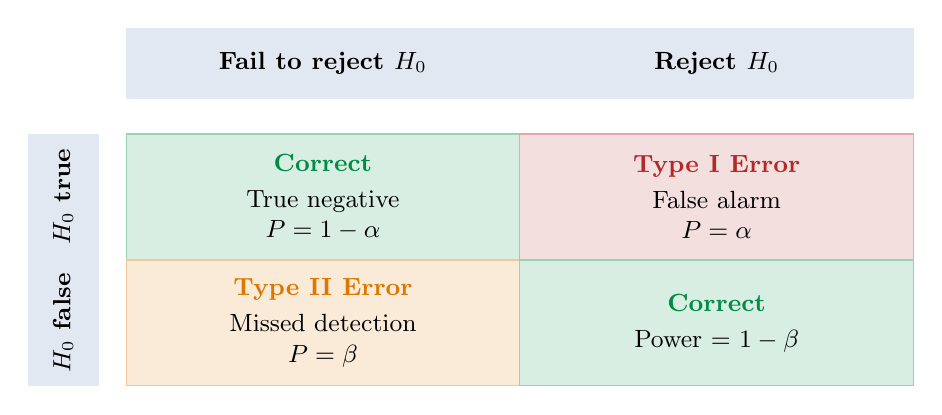
\begin{tikzpicture}[
  cell/.style={minimum width=5cm, minimum height=1.6cm, align=center, font=\small, inner sep=5pt},
  header/.style={minimum width=5cm, minimum height=0.9cm, align=center, font=\small\bfseries, inner sep=5pt}
]
  % Headers
  \node[header, fill=popblue!15] at (2.5, 2.5) {Fail to reject $H_0$};
  \node[header, fill=popblue!15] at (7.5, 2.5) {Reject $H_0$};
  \node[header, fill=popblue!15, rotate=90, minimum width=1.6cm] at (-0.8, 0.8) {$H_0$ true};
  \node[header, fill=popblue!15, rotate=90, minimum width=1.6cm] at (-0.8, -0.8) {$H_0$ false};

  % Cells
  \node[cell, fill=paramgreen!15, draw=paramgreen!40] at (2.5, 0.8) {
    \textcolor{paramgreen}{\textbf{Correct}}\\[2pt]
    True negative\\
    $P = 1 - \alpha$
  };
  \node[cell, fill=warnred!15, draw=warnred!40] at (7.5, 0.8) {
    \textcolor{warnred}{\textbf{Type I Error}}\\[2pt]
    False alarm\\
    $P = \alpha$
  };
  \node[cell, fill=orange1!15, draw=orange1!40] at (2.5, -0.8) {
    \textcolor{orange1}{\textbf{Type II Error}}\\[2pt]
    Missed detection\\
    $P = \beta$
  };
  \node[cell, fill=paramgreen!15, draw=paramgreen!40] at (7.5, -0.8) {
    \textcolor{paramgreen}{\textbf{Correct}}\\[2pt]
    Power = $1 - \beta$
  };
\end{tikzpicture}
\end{center}

\pause
\vspace{0.1cm}
\begin{center}
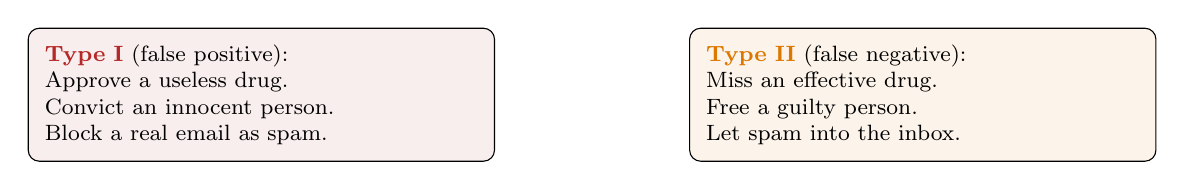
\begin{tikzpicture}[
  ebox/.style={draw, rounded corners=4pt, text width=5.5cm, align=left, inner sep=6pt, font=\footnotesize}
]
  \node[ebox, fill=warnred!8] at (-4.2, 0) {
    \textbf{\textcolor{warnred}{Type I}} (false positive):\\
    Approve a useless drug.\\
    Convict an innocent person.\\
    Block a real email as spam.
  };
  \node[ebox, fill=orange1!8] at (4.2, 0) {
    \textbf{\textcolor{orange1}{Type II}} (false negative):\\
    Miss an effective drug.\\
    Free a guilty person.\\
    Let spam into the inbox.
  };
\end{tikzpicture}
\end{center}
\end{frame}

% ============================================================
% PART III: p-VALUES
% ============================================================
\section{p-Values}

\begin{frame}
\begin{center}
  \vspace{1.5cm}
  {\Huge\bfseries\textcolor{popblue}{Part III: The p-Value}}

  \vspace{0.8cm}
  {\large The most used --- and most abused --- number in science}
\end{center}
\end{frame}

\begin{frame}
\frametitle{The p-Value: Definition}

\begin{center}
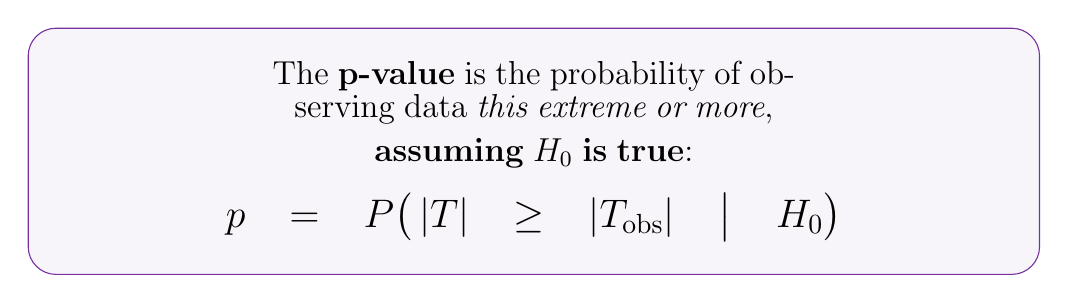
\begin{tikzpicture}
  \node[draw=violet1, fill=violet1!5, rounded corners=10pt, text width=12cm, align=center, inner sep=12pt] {
    {\large The \textbf{p-value} is the probability of observing data \textit{this extreme or more},}\\[4pt]
    {\large \textbf{assuming $H_0$ is true}:}\\[8pt]
    {\Large $p = P\bigl(\,|T| \geq |T_{\text{obs}}|\;\big|\;H_0\bigr)$}
  };
\end{tikzpicture}
\end{center}

\vspace{0.15cm}
\begin{center}
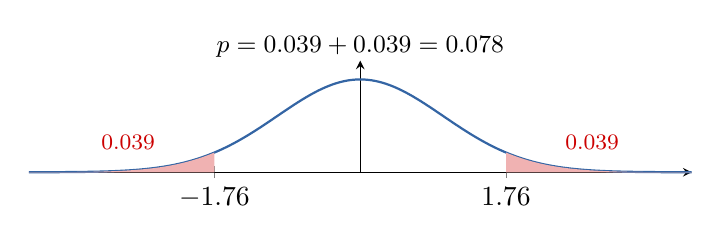
\begin{tikzpicture}
  \begin{axis}[
    width=10cm, height=3cm,
    domain=-4:4, samples=200,
    axis lines=middle,
    xtick={-1.76, 0, 1.76},
    xticklabels={$-1.76$, $0$, $1.76$},
    ytick=\empty,
    ymin=0, ymax=0.48,
    every axis plot/.style={thick, no markers},
    clip=false
  ]
    \addplot[popblue, thick] {exp(-0.5*x^2)/sqrt(2*pi)};
    \addplot[fill=sampred!30, draw=none, domain=-4:-1.76] {exp(-0.5*x^2)/sqrt(2*pi)} \closedcycle;
    \addplot[fill=sampred!30, draw=none, domain=1.76:4] {exp(-0.5*x^2)/sqrt(2*pi)} \closedcycle;
    \node[font=\footnotesize\bfseries, sampred] at (axis cs:-2.8, 0.13) {$0.039$};
    \node[font=\footnotesize\bfseries, sampred] at (axis cs:2.8, 0.13) {$0.039$};
    \node[font=\small\bfseries, above] at (axis cs:0, 0.45) {$p = 0.039 + 0.039 = 0.078$};
  \end{axis}
\end{tikzpicture}
\end{center}

\vspace{0.1cm}
\small Drug trial: $p = 0.078 > 0.05 = \alpha$ $\;\Rightarrow\;$ fail to reject $H_0$.\\
\textbf{Rule:} Reject $H_0$ if and only if $p \leq \alpha$.
\end{frame}

\begin{frame}
\frametitle{What the p-Value Is NOT}

\begin{center}
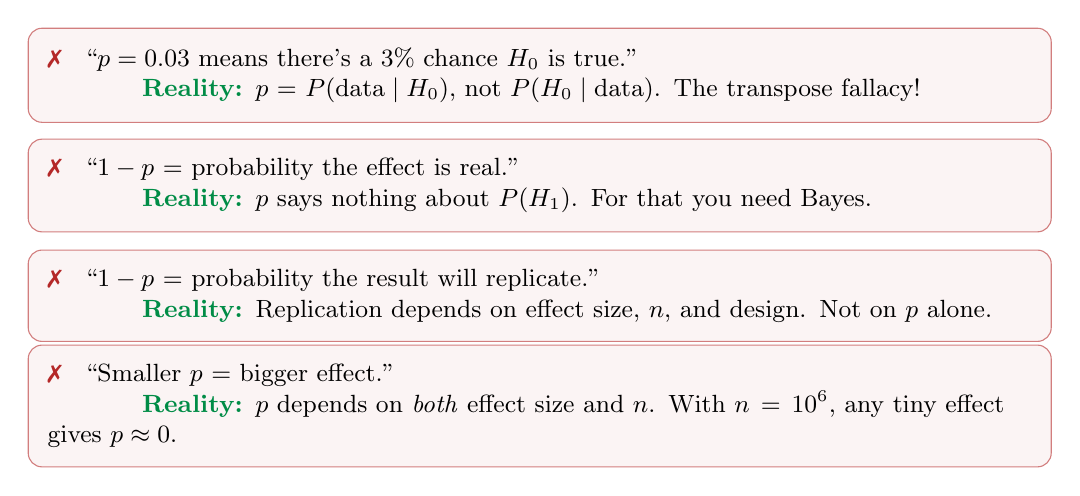
\begin{tikzpicture}[
  mbox/.style={draw=warnred!60, fill=warnred!5, rounded corners=5pt, text width=12.5cm, align=left, inner sep=7pt, font=\small}
]
  \node[mbox] at (0, 2.4) {
    \textcolor{warnred}{\textbf{\ding{55}}} \;\;``$p = 0.03$ means there's a 3\% chance $H_0$ is true.''\\
    \hspace{1.2cm}\textcolor{paramgreen}{\textbf{Reality:}} $p$ = $P(\text{data} \mid H_0)$, not $P(H_0 \mid \text{data})$.
    The transpose fallacy!
  };

  \pause
  \node[mbox] at (0, 1.0) {
    \textcolor{warnred}{\textbf{\ding{55}}} \;\;``$1 - p$ = probability the effect is real.''\\
    \hspace{1.2cm}\textcolor{paramgreen}{\textbf{Reality:}} $p$ says nothing about $P(H_1)$. For that you need Bayes.
  };

  \pause
  \node[mbox] at (0, -0.4) {
    \textcolor{warnred}{\textbf{\ding{55}}} \;\;``$1 - p$ = probability the result will replicate.''\\
    \hspace{1.2cm}\textcolor{paramgreen}{\textbf{Reality:}} Replication depends on effect size, $n$, and design. Not on $p$ alone.
  };

  \pause
  \node[mbox] at (0, -1.8) {
    \textcolor{warnred}{\textbf{\ding{55}}} \;\;``Smaller $p$ = bigger effect.''\\
    \hspace{1.2cm}\textcolor{paramgreen}{\textbf{Reality:}} $p$ depends on \textit{both} effect size and $n$. With $n = 10^6$, any tiny effect gives $p \approx 0$.
  };
\end{tikzpicture}
\end{center}
\end{frame}

\begin{frame}
\frametitle{Statistical vs Practical Significance}

\small
With enough data, \textit{any} nonzero effect becomes ``statistically significant.''

\vspace{0.2cm}
\begin{center}
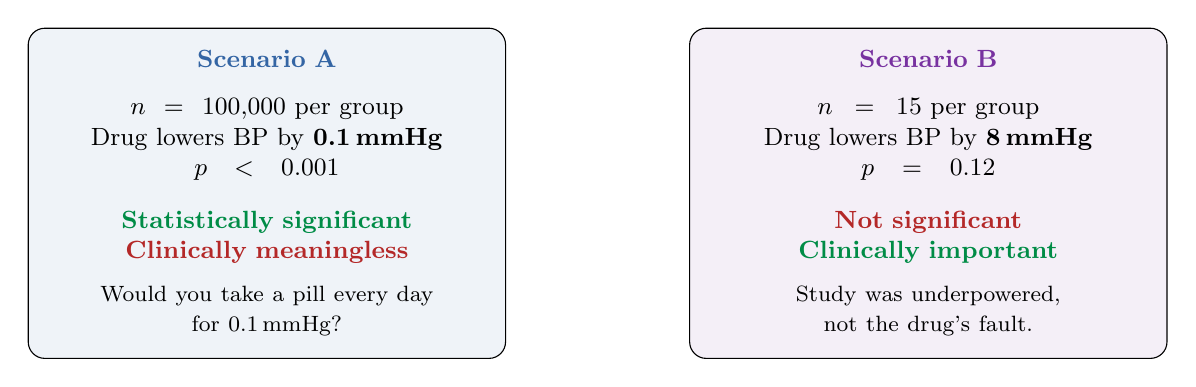
\begin{tikzpicture}[
  cbox/.style={draw, rounded corners=6pt, text width=5.5cm, align=center, inner sep=8pt, font=\small, minimum height=4cm}
]
  \node[cbox, fill=popblue!8] at (-4.2, 0) {
    \textbf{\textcolor{popblue}{Scenario A}}\\[6pt]
    $n = 100{,}000$ per group\\
    Drug lowers BP by \textbf{0.1\,mmHg}\\
    $p < 0.001$\\[8pt]
    \textcolor{paramgreen}{\textbf{Statistically significant}}\\
    \textcolor{warnred}{\textbf{Clinically meaningless}}\\[6pt]
    \footnotesize Would you take a pill every day\\
    for 0.1\,mmHg?
  };

  \node[cbox, fill=violet1!8] at (4.2, 0) {
    \textbf{\textcolor{violet1}{Scenario B}}\\[6pt]
    $n = 15$ per group\\
    Drug lowers BP by \textbf{8\,mmHg}\\
    $p = 0.12$\\[8pt]
    \textcolor{warnred}{\textbf{Not significant}}\\
    \textcolor{paramgreen}{\textbf{Clinically important}}\\[6pt]
    \footnotesize Study was underpowered,\\
    not the drug's fault.
  };
\end{tikzpicture}
\end{center}

\vspace{0.15cm}
\begin{center}
\fcolorbox{orange1}{orange1!5}{\parbox{10cm}{\centering\small
  Always report: \textbf{(1) effect size}, \textbf{(2) confidence interval}, \textbf{(3) p-value}.\\
  Ask ``\textbf{How big} is the effect?'', not just ``Is it nonzero?''
}}
\end{center}
\end{frame}

\begin{frame}
\frametitle{$p = 0.049$ vs $p = 0.051$}

\begin{center}
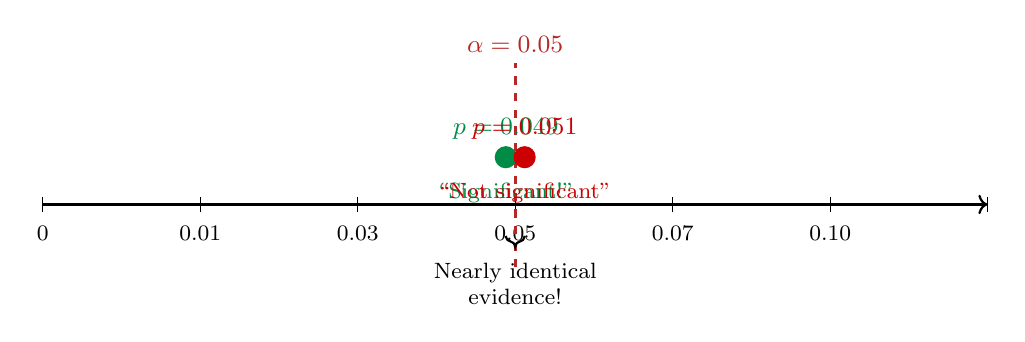
\begin{tikzpicture}
  % Number line
  \draw[thick, ->] (0, 0) -- (12, 0);
  \foreach \x/\lab in {0/0, 2/0.01, 4/0.03, 6/0.05, 8/0.07, 10/0.10, 12/} {
    \draw (\x, -0.1) -- (\x, 0.1);
    \node[font=\footnotesize, below] at (\x, -0.15) {\lab};
  }

  % Threshold
  \draw[very thick, dashed, warnred] (6, -0.8) -- (6, 1.8);
  \node[font=\small\bfseries, warnred, above] at (6, 1.8) {$\alpha = 0.05$};

  % Two studies
  \fill[paramgreen] (5.88, 0.6) circle (4pt);
  \node[font=\small, paramgreen, above] at (5.88, 0.7) {$p = 0.049$};
  \node[font=\footnotesize, paramgreen, below] at (5.88, 0.4) {``Significant!''};

  \fill[sampred] (6.12, 0.6) circle (4pt);
  \node[font=\small, sampred, above] at (6.12, 0.7) {$p = 0.051$};
  \node[font=\footnotesize, sampred, below] at (6.12, 0.4) {``Not significant''};

  % Brace
  \draw[thick, decorate, decoration={brace, amplitude=4pt, mirror}] (5.88, -0.4) -- (6.12, -0.4)
    node[midway, below=6pt, font=\footnotesize, align=center] {Nearly identical\\evidence!};
\end{tikzpicture}
\end{center}

\pause
\vspace{0.3cm}
\begin{center}
\fcolorbox{orange1}{orange1!5}{\parbox{11cm}{\centering\small
  The 0.05 threshold is a \textbf{convention}, not a law of nature.\\[2pt]
  \textbf{ASA (2016):} ``Scientific conclusions should not be based only on\\
  whether a p-value passes a specific threshold.''
}}
\end{center}
\end{frame}

% ============================================================
% PART IV: POWER ANALYSIS
% ============================================================
\section{Power and Sample Size}

\begin{frame}
\begin{center}
  \vspace{1.5cm}
  {\Huge\bfseries\textcolor{popblue}{Part IV: Power Analysis}}

  \vspace{0.8cm}
  {\large How to design a study that can actually find what you're looking for}
\end{center}
\end{frame}

\begin{frame}
\frametitle{Power: The Ability to Detect Real Effects}

\begin{center}
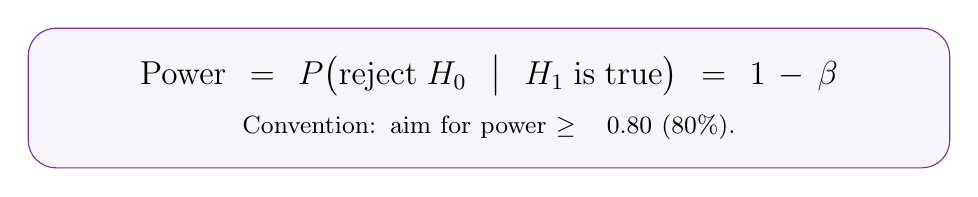
\begin{tikzpicture}
  \node[draw=violet1, fill=violet1!5, rounded corners=10pt, text width=11cm, align=center, inner sep=10pt] {
    {\large $\text{Power} = P\bigl(\text{reject } H_0 \;\big|\; H_1 \text{ is true}\bigr) = 1 - \beta$}\\[6pt]
    \small Convention: aim for power $\geq 0.80$ (80\%).
  };
\end{tikzpicture}
\end{center}

\vspace{0.15cm}
\begin{center}
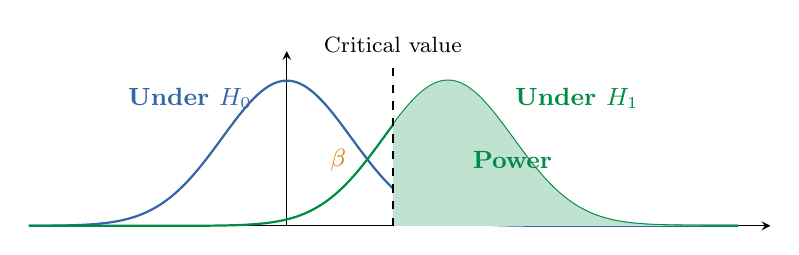
\begin{tikzpicture}
  \begin{axis}[
    width=11cm, height=3.8cm,
    domain=-4:7, samples=200,
    axis lines=middle,
    xtick=\empty, ytick=\empty,
    ymin=0, ymax=0.48,
    xmin=-4, xmax=7.5,
    every axis plot/.style={thick, no markers},
    clip=false
  ]
    % H0 distribution
    \addplot[popblue, thick] {exp(-0.5*x^2)/sqrt(2*pi)};
    \addplot[fill=warnred!25, draw=none, domain=1.645:4] {exp(-0.5*x^2)/sqrt(2*pi)} \closedcycle;
    \node[font=\small\bfseries, popblue] at (axis cs:-1.5, 0.35) {Under $H_0$};
    \node[font=\tiny, warnred] at (axis cs:2.5, 0.08) {$\alpha$};

    % H1 distribution (shifted by delta=2.5)
    \addplot[paramgreen, thick] {exp(-0.5*(x-2.5)^2)/sqrt(2*pi)};
    \addplot[fill=paramgreen!25, draw=none, domain=1.645:7] {exp(-0.5*(x-2.5)^2)/sqrt(2*pi)} \closedcycle;
    \node[font=\small\bfseries, paramgreen] at (axis cs:4.5, 0.35) {Under $H_1$};

    % Power label
    \node[font=\small\bfseries, paramgreen] at (axis cs:3.5, 0.18) {Power};
    \node[font=\small, orange1] at (axis cs:0.8, 0.18) {$\beta$};

    % Critical value line
    \draw[thick, dashed, black] (axis cs:1.645, 0) -- (axis cs:1.645, 0.45);
    \node[font=\footnotesize, above] at (axis cs:1.645, 0.45) {Critical value};
  \end{axis}
\end{tikzpicture}
\end{center}
\end{frame}

\begin{frame}
\frametitle{What Determines Power?}

\begin{center}
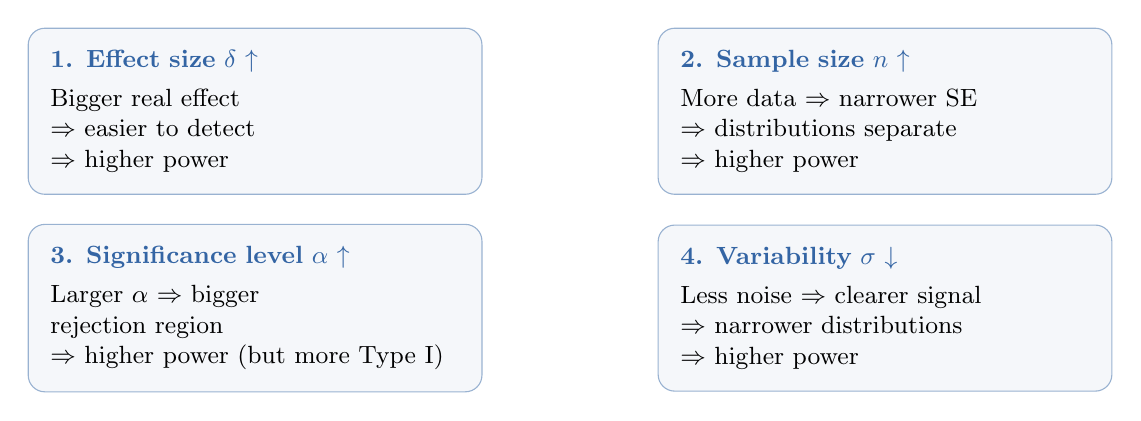
\begin{tikzpicture}[
  wbox/.style={draw=popblue!50, fill=popblue!5, rounded corners=6pt, text width=5.2cm, minimum height=1.8cm, align=left, inner sep=8pt, font=\small}
]
  \node[wbox] at (-4, 1.5) {
    \textbf{\textcolor{popblue}{1. Effect size $\delta$ $\uparrow$}}\\[3pt]
    Bigger real effect\\
    $\Rightarrow$ easier to detect\\
    $\Rightarrow$ higher power
  };
  \node[wbox] at (4, 1.5) {
    \textbf{\textcolor{popblue}{2. Sample size $n$ $\uparrow$}}\\[3pt]
    More data $\Rightarrow$ narrower SE\\
    $\Rightarrow$ distributions separate\\
    $\Rightarrow$ higher power
  };
  \node[wbox] at (-4, -1.0) {
    \textbf{\textcolor{popblue}{3. Significance level $\alpha$ $\uparrow$}}\\[3pt]
    Larger $\alpha$ $\Rightarrow$ bigger\\
    rejection region\\
    $\Rightarrow$ higher power (but more Type~I)
  };
  \node[wbox] at (4, -1.0) {
    \textbf{\textcolor{popblue}{4. Variability $\sigma$ $\downarrow$}}\\[3pt]
    Less noise $\Rightarrow$ clearer signal\\
    $\Rightarrow$ narrower distributions\\
    $\Rightarrow$ higher power
  };
\end{tikzpicture}
\end{center}

\vspace{0.15cm}
\begin{center}
\fcolorbox{orange1}{orange1!5}{\parbox{10cm}{\centering\small
  You control \textbf{$n$} and \textbf{$\alpha$}. Nature controls \textbf{$\delta$} and \textbf{$\sigma$}.\\
  Power analysis = choosing $n$ so that you can detect a meaningful $\delta$.
}}
\end{center}
\end{frame}

\begin{frame}
\frametitle{Effect Size: Cohen's $d$}

\begin{center}
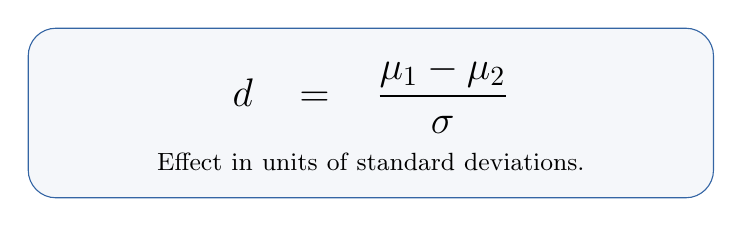
\begin{tikzpicture}
  \node[draw=popblue, fill=popblue!5, rounded corners=10pt, text width=8cm, align=center, inner sep=10pt] {
    {\Large $d = \dfrac{\mu_1 - \mu_2}{\sigma}$}\\[6pt]
    \small Effect in units of standard deviations.
  };
\end{tikzpicture}
\end{center}

\vspace{0.15cm}
\begin{center}
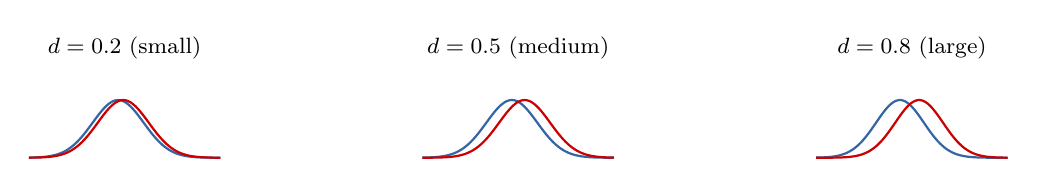
\begin{tikzpicture}
  % Small effect d=0.2
  \begin{scope}[xshift=0cm]
    \begin{axis}[
      width=4.5cm, height=2.5cm,
      domain=-3.5:4, samples=80,
      axis lines=none, ticks=none,
      ymin=0, ymax=0.5,
      clip=false, title={\footnotesize $d = 0.2$ (small)}
    ]
      \addplot[popblue, thick] {exp(-0.5*x^2)/sqrt(2*pi)};
      \addplot[sampred, thick] {exp(-0.5*(x-0.2)^2)/sqrt(2*pi)};
    \end{axis}
  \end{scope}
  % Medium effect d=0.5
  \begin{scope}[xshift=5cm]
    \begin{axis}[
      width=4.5cm, height=2.5cm,
      domain=-3.5:4, samples=80,
      axis lines=none, ticks=none,
      ymin=0, ymax=0.5,
      clip=false, title={\footnotesize $d = 0.5$ (medium)}
    ]
      \addplot[popblue, thick] {exp(-0.5*x^2)/sqrt(2*pi)};
      \addplot[sampred, thick] {exp(-0.5*(x-0.5)^2)/sqrt(2*pi)};
    \end{axis}
  \end{scope}
  % Large effect d=0.8
  \begin{scope}[xshift=10cm]
    \begin{axis}[
      width=4.5cm, height=2.5cm,
      domain=-3.5:4.5, samples=80,
      axis lines=none, ticks=none,
      ymin=0, ymax=0.5,
      clip=false, title={\footnotesize $d = 0.8$ (large)}
    ]
      \addplot[popblue, thick] {exp(-0.5*x^2)/sqrt(2*pi)};
      \addplot[sampred, thick] {exp(-0.5*(x-0.8)^2)/sqrt(2*pi)};
    \end{axis}
  \end{scope}
\end{tikzpicture}
\end{center}

\vspace{0.1cm}
\small
Drug trial: $d = 3/12 = 0.25$ (small).\\
Effect size is \textbf{independent of sample size} --- it measures the \textit{phenomenon}, not the study.
\end{frame}

\begin{frame}
\frametitle{Power Curves: Planning Your Study}
\framesubtitle{Two-sample $z$-test, $\alpha = 0.05$, two-sided}

\begin{center}
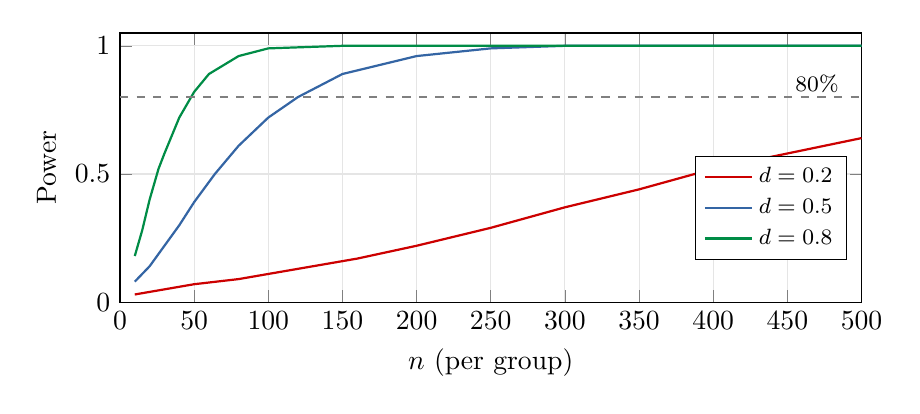
\begin{tikzpicture}
  \begin{axis}[
    width=11cm, height=5cm,
    xlabel={$n$ (per group)},
    ylabel={Power},
    xmin=0, xmax=500,
    ymin=0, ymax=1.05,
    grid=major,
    grid style={gray!20},
    legend style={at={(0.98,0.35)}, anchor=east, font=\footnotesize},
    every axis plot/.style={thick, no markers}
  ]
    % d=0.2: Power = Phi(0.2*sqrt(n/2) - 1.96)
    \addplot[sampred] coordinates {
      (10,0.03)(30,0.05)(50,0.07)(80,0.09)(100,0.11)(130,0.14)(160,0.17)
      (200,0.22)(250,0.29)(300,0.37)(350,0.44)(400,0.52)(450,0.58)(500,0.64)
    };
    \addlegendentry{$d = 0.2$}
    % d=0.5: Power = Phi(0.5*sqrt(n/2) - 1.96)
    \addplot[popblue] coordinates {
      (10,0.08)(20,0.14)(30,0.22)(40,0.30)(50,0.39)(64,0.50)(80,0.61)
      (100,0.72)(120,0.80)(150,0.89)(200,0.96)(250,0.99)(300,1.0)(500,1.0)
    };
    \addlegendentry{$d = 0.5$}
    % d=0.8: Power = Phi(0.8*sqrt(n/2) - 1.96)
    \addplot[paramgreen] coordinates {
      (10,0.18)(15,0.28)(20,0.40)(26,0.52)(30,0.58)(40,0.72)(50,0.82)
      (60,0.89)(80,0.96)(100,0.99)(150,1.0)(200,1.0)(300,1.0)(500,1.0)
    };
    \addlegendentry{$d = 0.8$}
    % 80% power line
    \draw[thick, dashed, black!50] (axis cs:0, 0.8) -- (axis cs:500, 0.8);
    \node[font=\footnotesize] at (axis cs:470, 0.85) {80\%};
  \end{axis}
\end{tikzpicture}
\end{center}

\vspace{0.1cm}
\small
Required $n$ per group for 80\% power: \;
$d = 0.8$: $n \approx 26$ \quad
$d = 0.5$: $n \approx 64$ \quad
$d = 0.2$: $n \approx 394$
\end{frame}

\begin{frame}
\frametitle{Sample Size Formula}

\begin{center}
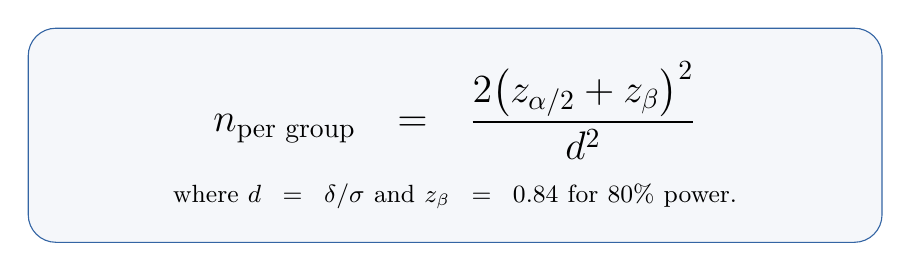
\begin{tikzpicture}
  \node[draw=popblue, fill=popblue!5, rounded corners=10pt, text width=10cm, align=center, inner sep=12pt] {
    {\Large $n_{\text{per group}} = \dfrac{2\bigl(z_{\alpha/2} + z_\beta\bigr)^2}{d^2}$}\\[8pt]
    \small where $d = \delta/\sigma$ and $z_\beta = 0.84$ for 80\% power.
  };
\end{tikzpicture}
\end{center}

\vspace{0.3cm}
\begin{center}
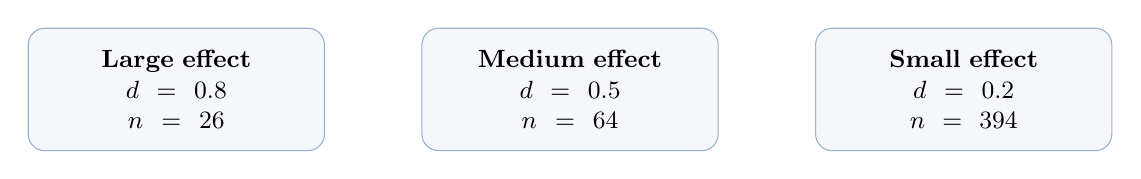
\begin{tikzpicture}[
  nbox/.style={draw=popblue!50, fill=popblue!5, rounded corners=6pt, text width=3.2cm, align=center, inner sep=8pt, font=\small, minimum height=1.5cm}
]
  \node[nbox] at (-5, 0) {\textbf{Large effect}\\$d = 0.8$\\$n = 26$};
  \node[nbox] at (0, 0) {\textbf{Medium effect}\\$d = 0.5$\\$n = 64$};
  \node[nbox] at (5, 0) {\textbf{Small effect}\\$d = 0.2$\\$n = 394$};
\end{tikzpicture}
\end{center}

\vspace{0.3cm}
\begin{center}
\fcolorbox{orange1}{orange1!5}{\parbox{11cm}{\centering\small
  \textbf{An underpowered study wastes resources.} If you can only recruit 50 patients,\\
  you can only detect $d \geq 0.57$. Know this \textit{before} you start collecting data.
}}
\end{center}
\end{frame}

% ============================================================
% PART V: PERMUTATION TESTS
% ============================================================
\section{Permutation Tests}

\begin{frame}
\begin{center}
  \vspace{1.5cm}
  {\Huge\bfseries\textcolor{popblue}{Part V: Permutation Tests}}

  \vspace{0.8cm}
  {\large No distributional assumptions --- let the data speak}
\end{center}
\end{frame}

\begin{frame}
\frametitle{If $H_0$ Is True, Labels Don't Matter}

\small
Under $H_0$: drug and placebo groups come from the \textit{same} distribution.\\
So the group labels are \textbf{arbitrary} --- shuffling them shouldn't change anything.

\vspace{0.2cm}
\begin{center}
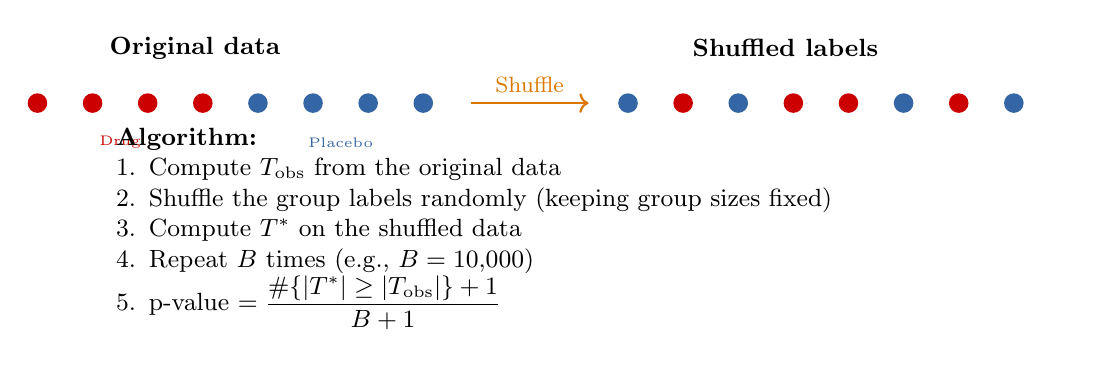
\begin{tikzpicture}[
  pt/.style={circle, inner sep=2.5pt, minimum size=5pt}
]
  % Original
  \node[font=\small\bfseries] at (0, 2.5) {Original data};
  \foreach \x/\col in {-2/sampred, -1.3/sampred, -0.6/sampred, 0.1/sampred, 0.8/popblue, 1.5/popblue, 2.2/popblue, 2.9/popblue} {
    \node[pt, fill=\col] at (\x, 1.8) {};
  }
  \node[font=\tiny, sampred] at (-0.95, 1.3) {Drug};
  \node[font=\tiny, popblue] at (1.85, 1.3) {Placebo};

  % Arrow
  \draw[->, thick, orange1] (3.5, 1.8) -- (5.0, 1.8) node[midway, above, font=\footnotesize] {Shuffle};

  % Shuffled 1
  \node[font=\small\bfseries] at (7.5, 2.5) {Shuffled labels};
  \foreach \x/\col in {5.5/popblue, 6.2/sampred, 6.9/popblue, 7.6/sampred, 8.3/sampred, 9.0/popblue, 9.7/sampred, 10.4/popblue} {
    \node[pt, fill=\col] at (\x, 1.8) {};
  }

  % Algorithm sketch
  \node[font=\small, align=left, text width=12cm] at (5, 0.2) {
    \textbf{Algorithm:}\\
    1. Compute $T_{\text{obs}}$ from the original data\\
    2. Shuffle the group labels randomly (keeping group sizes fixed)\\
    3. Compute $T^*$ on the shuffled data\\
    4. Repeat $B$ times (e.g., $B = 10{,}000$)\\
    5. p-value $= \dfrac{\#\{|T^*| \geq |T_{\text{obs}}|\} + 1}{B + 1}$
  };
\end{tikzpicture}
\end{center}
\end{frame}

\begin{frame}
\frametitle{Permutation Distribution}
\framesubtitle{Drug trial: $T_{\text{obs}} = -1.76$, $B = 10{,}000$ permutations}

\begin{center}
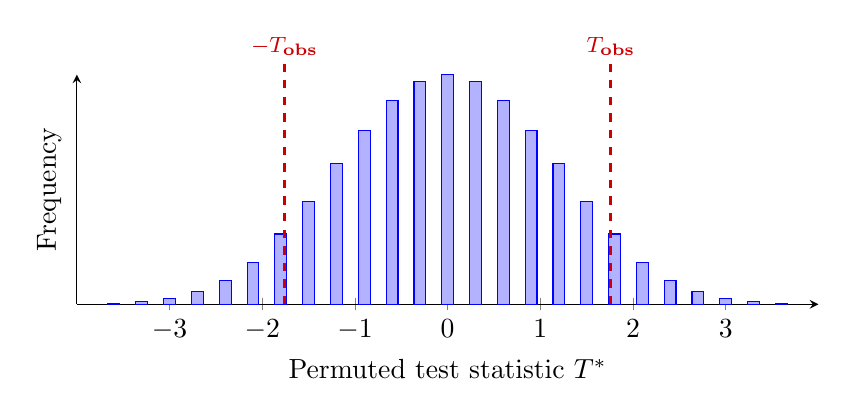
\begin{tikzpicture}
  \begin{axis}[
    width=11cm, height=4.5cm,
    ybar,
    bar width=0.15cm,
    xlabel={Permuted test statistic $T^*$},
    ylabel={Frequency},
    xmin=-4, xmax=4,
    ymin=0,
    xtick={-3,-2,-1,0,1,2,3},
    ytick=\empty,
    axis lines=left,
    every axis plot/.style={fill=popblue!40, draw=popblue!60},
    clip=false
  ]
    % Approximate histogram of N(0,1) * 10000 with bin width 0.3
    \addplot coordinates {
      (-3.6, 5) (-3.3, 12) (-3.0, 25) (-2.7, 55) (-2.4, 100)
      (-2.1, 180) (-1.8, 300) (-1.5, 440) (-1.2, 600) (-0.9, 740)
      (-0.6, 870) (-0.3, 950) (0.0, 980) (0.3, 950) (0.6, 870)
      (0.9, 740) (1.2, 600) (1.5, 440) (1.8, 300) (2.1, 180)
      (2.4, 100) (2.7, 55) (3.0, 25) (3.3, 12) (3.6, 5)
    };

    % Observed T
    \draw[very thick, dashed, sampred] (axis cs:-1.76, 0) -- (axis cs:-1.76, 1050);
    \draw[very thick, dashed, sampred] (axis cs:1.76, 0) -- (axis cs:1.76, 1050);
    \node[font=\footnotesize\bfseries, sampred] at (axis cs:-1.76, 1100) {$-T_{\text{obs}}$};
    \node[font=\footnotesize\bfseries, sampred] at (axis cs:1.76, 1100) {$T_{\text{obs}}$};
  \end{axis}
\end{tikzpicture}
\end{center}

\vspace{0.1cm}
\small
Count: $\approx 780$ of $10{,}000$ permutations have $|T^*| \geq 1.76$.\\
Permutation $p$-value: $\approx 0.078$ --- nearly identical to the $z$-test $p = 0.078$.
\end{frame}

\begin{frame}
\frametitle{Permutation Tests: Pros and Cons}

\begin{center}
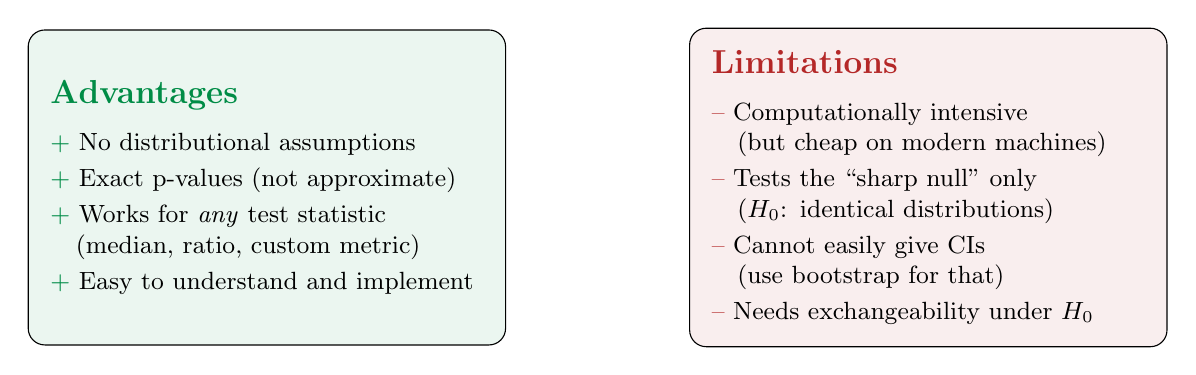
\begin{tikzpicture}[
  cbox/.style={draw, rounded corners=6pt, minimum height=4cm, text width=5.5cm, align=left, inner sep=8pt, font=\small}
]
  \node[cbox, fill=paramgreen!8] at (-4.2, 0) {
    \textbf{\large\textcolor{paramgreen}{Advantages}}\\[6pt]
    \textcolor{paramgreen}{+} No distributional assumptions\\[2pt]
    \textcolor{paramgreen}{+} Exact p-values (not approximate)\\[2pt]
    \textcolor{paramgreen}{+} Works for \textit{any} test statistic\\
    \quad (median, ratio, custom metric)\\[2pt]
    \textcolor{paramgreen}{+} Easy to understand and implement
  };

  \node[cbox, fill=warnred!8] at (4.2, 0) {
    \textbf{\large\textcolor{warnred}{Limitations}}\\[6pt]
    \textcolor{warnred}{--} Computationally intensive\\
    \quad (but cheap on modern machines)\\[2pt]
    \textcolor{warnred}{--} Tests the ``sharp null'' only\\
    \quad ($H_0$: identical distributions)\\[2pt]
    \textcolor{warnred}{--} Cannot easily give CIs\\
    \quad (use bootstrap for that)\\[2pt]
    \textcolor{warnred}{--} Needs exchangeability under $H_0$
  };
\end{tikzpicture}
\end{center}
\end{frame}

% ============================================================
% PART VI: MULTIPLE TESTING
% ============================================================
\section{Multiple Testing}

\begin{frame}
\begin{center}
  \vspace{1.5cm}
  {\Huge\bfseries\textcolor{popblue}{Part VI: Multiple Testing}}

  \vspace{0.8cm}
  {\large Test 20 hypotheses, and one will be ``significant'' by chance}
\end{center}
\end{frame}

\begin{frame}
\frametitle{The Multiple Testing Problem}

\small
If you test $m = 20$ independent true nulls at $\alpha = 0.05$:

\vspace{0.1cm}
\begin{center}
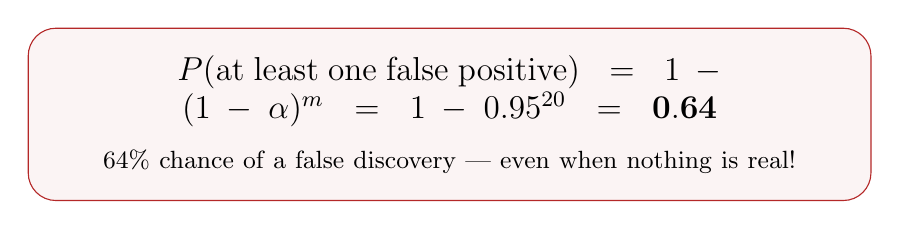
\begin{tikzpicture}
  \node[draw=warnred, fill=warnred!5, rounded corners=10pt, text width=10cm, align=center, inner sep=10pt] {
    {\large $P(\text{at least one false positive}) = 1 - (1 - \alpha)^m = 1 - 0.95^{20} = \mathbf{0.64}$}\\[6pt]
    \small 64\% chance of a false discovery --- even when nothing is real!
  };
\end{tikzpicture}
\end{center}

\vspace{0.15cm}
\begin{center}
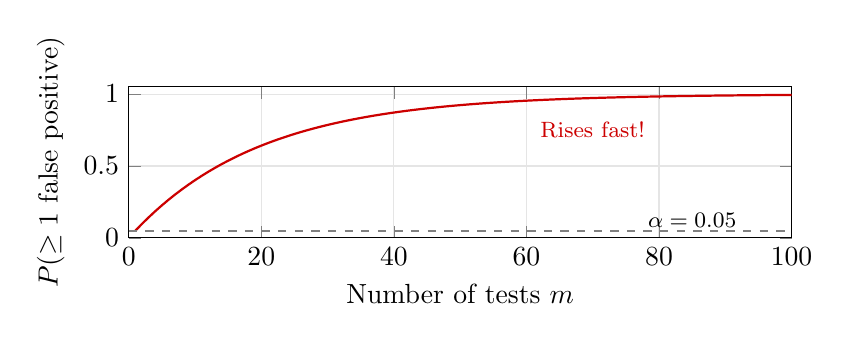
\begin{tikzpicture}
  \begin{axis}[
    width=10cm, height=3.5cm,
    xlabel={Number of tests $m$},
    ylabel={$P(\geq 1$ false positive$)$},
    xmin=0, xmax=100,
    ymin=0, ymax=1.05,
    grid=major, grid style={gray!20},
    every axis plot/.style={thick, no markers, samples=100, domain=1:100}
  ]
    \addplot[sampred, thick] {1 - (0.95)^x};
    \draw[thick, dashed, black!50] (axis cs:0, 0.05) -- (axis cs:100, 0.05);
    \node[font=\footnotesize] at (axis cs:85, 0.12) {$\alpha = 0.05$};
    \node[font=\footnotesize, sampred] at (axis cs:70, 0.75) {Rises fast!};
  \end{axis}
\end{tikzpicture}
\end{center}

\vspace{0.1cm}
\small Examples: 20{,}000 genes, 50 A/B test variants, multiple clinical endpoints.
\end{frame}

\begin{frame}
\frametitle{Bonferroni vs Benjamini--Hochberg}

\begin{center}
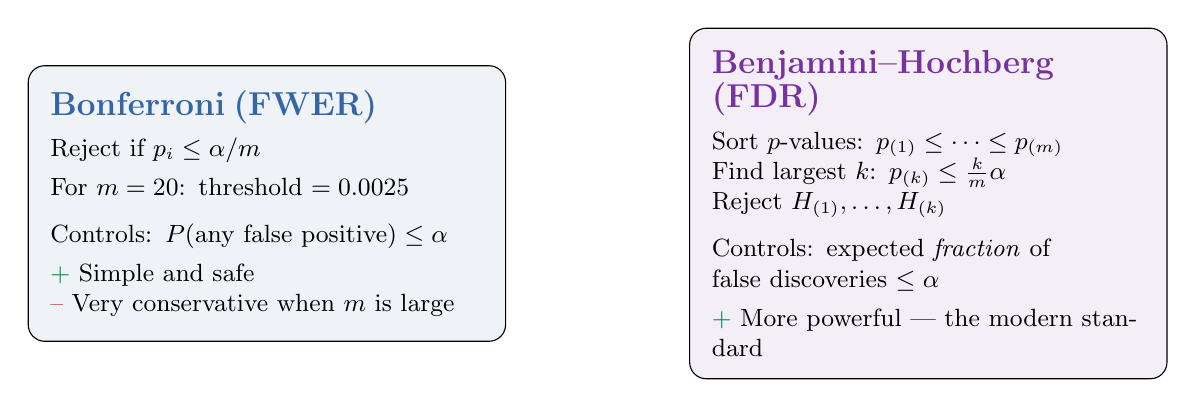
\begin{tikzpicture}[
  cbox/.style={draw, rounded corners=6pt, minimum height=3.5cm, text width=5.5cm, align=left, inner sep=8pt, font=\small}
]
  \node[cbox, fill=popblue!8] at (-4.2, 0.2) {
    \textbf{\large\textcolor{popblue}{Bonferroni (FWER)}}\\[4pt]
    Reject if $p_i \leq \alpha / m$\\[3pt]
    For $m = 20$: threshold $= 0.0025$\\[6pt]
    Controls: $P(\text{any false positive}) \leq \alpha$\\[3pt]
    \textcolor{paramgreen}{+} Simple and safe\\
    \textcolor{warnred}{--} Very conservative when $m$ is large
  };

  \node[cbox, fill=violet1!8] at (4.2, 0.2) {
    \textbf{\large\textcolor{violet1}{Benjamini--Hochberg (FDR)}}\\[4pt]
    Sort $p$-values: $p_{(1)} \leq \cdots \leq p_{(m)}$\\
    Find largest $k$: $p_{(k)} \leq \frac{k}{m}\alpha$\\
    Reject $H_{(1)}, \ldots, H_{(k)}$\\[6pt]
    Controls: expected \textit{fraction} of\\
    false discoveries $\leq \alpha$\\[3pt]
    \textcolor{paramgreen}{+} More powerful --- the modern standard
  };
\end{tikzpicture}
\end{center}

\vspace{0.15cm}
\begin{center}
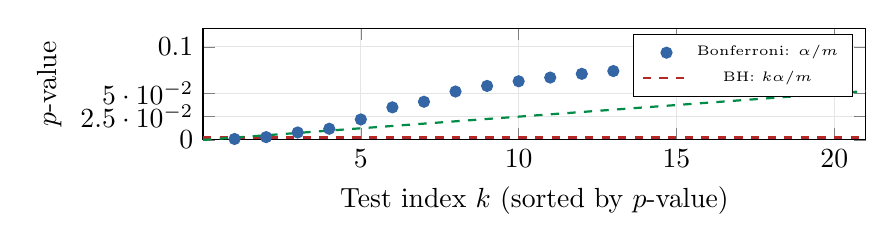
\begin{tikzpicture}
  \begin{axis}[
    width=10cm, height=3cm,
    xlabel={Test index $k$ (sorted by $p$-value)},
    ylabel={$p$-value},
    xmin=0, xmax=21,
    ymin=0, ymax=0.12,
    xtick={5,10,15,20},
    ytick={0, 0.025, 0.05, 0.1},
    grid=major, grid style={gray!20},
    legend style={at={(0.98,0.95)}, anchor=north east, font=\tiny},
    clip=false
  ]
    % Sorted p-values (some small, most large)
    \addplot[only marks, mark=*, mark size=2pt, popblue] coordinates {
      (1, 0.001) (2, 0.003) (3, 0.008) (4, 0.012) (5, 0.022)
      (6, 0.035) (7, 0.041) (8, 0.052) (9, 0.058) (10, 0.063)
      (11, 0.067) (12, 0.071) (13, 0.074) (14, 0.078) (15, 0.082)
      (16, 0.085) (17, 0.089) (18, 0.092) (19, 0.095) (20, 0.098)
    };
    % Bonferroni threshold
    \addplot[thick, dashed, warnred, domain=0:21] {0.0025};
    \addlegendentry{Bonferroni: $\alpha/m$}
    % BH threshold line
    \addplot[thick, dashed, paramgreen, domain=0:21] {x * 0.05 / 20};
    \addlegendentry{BH: $k\alpha/m$}
  \end{axis}
\end{tikzpicture}
\end{center}
\end{frame}

% ============================================================
\section{Summary}

\begin{frame}
\frametitle{Summary: Hypothesis Testing}
\begin{center}
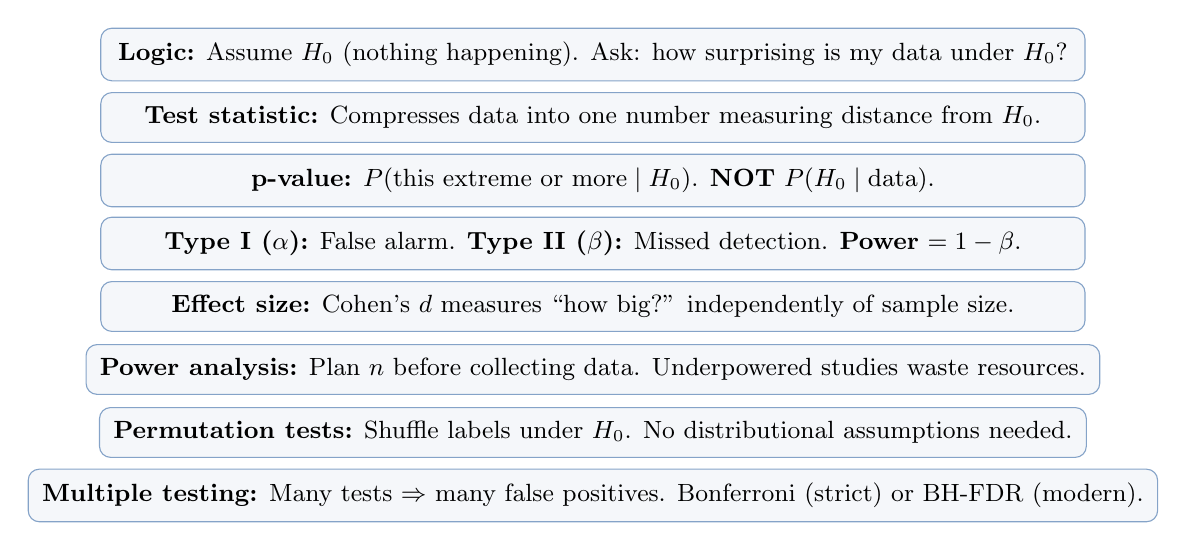
\begin{tikzpicture}[
  sbox/.style={draw=popblue!60, fill=popblue!5, rounded corners=4pt, minimum width=12.5cm, minimum height=0.5cm, align=left, inner sep=5pt, font=\small}
]
  \node[sbox] at (0, 3.2) {\textbf{Logic:} Assume $H_0$ (nothing happening). Ask: how surprising is my data under $H_0$?};
  \node[sbox] at (0, 2.4) {\textbf{Test statistic:} Compresses data into one number measuring distance from $H_0$.};
  \node[sbox] at (0, 1.6) {\textbf{p-value:} $P(\text{this extreme or more} \mid H_0)$. \textbf{NOT} $P(H_0 \mid \text{data})$.};
  \node[sbox] at (0, 0.8) {\textbf{Type I ($\alpha$):} False alarm. \textbf{Type II ($\beta$):} Missed detection. \textbf{Power} $= 1 - \beta$.};
  \node[sbox] at (0, 0.0) {\textbf{Effect size:} Cohen's $d$ measures ``how big?'' independently of sample size.};
  \node[sbox] at (0, -0.8) {\textbf{Power analysis:} Plan $n$ before collecting data. Underpowered studies waste resources.};
  \node[sbox] at (0, -1.6) {\textbf{Permutation tests:} Shuffle labels under $H_0$. No distributional assumptions needed.};
  \node[sbox] at (0, -2.4) {\textbf{Multiple testing:} Many tests $\Rightarrow$ many false positives. Bonferroni (strict) or BH-FDR (modern).};
\end{tikzpicture}
\end{center}
\end{frame}

% ============================================================
\section{Practical}

\begin{frame}
\frametitle{Practical: Hypothesis Testing \& Power}
\begin{center}
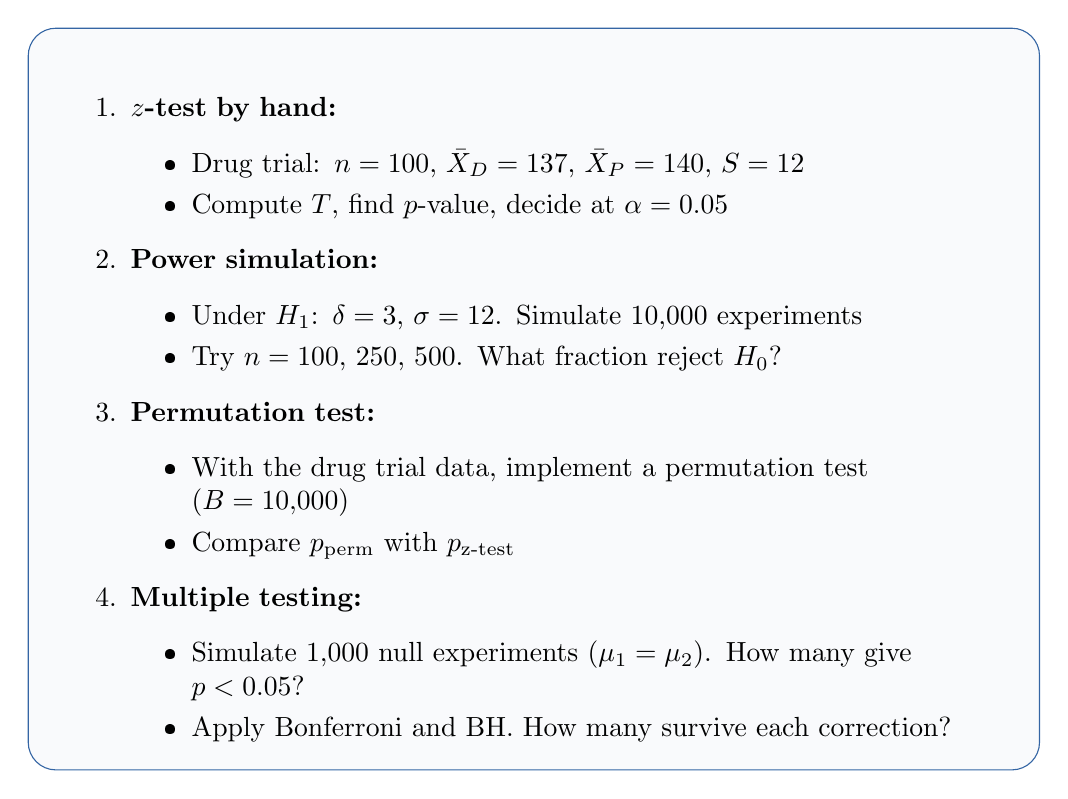
\begin{tikzpicture}
  \node[draw=popblue, fill=popblue!3, rounded corners=10pt, text width=12cm, align=left, inner sep=12pt] {
    \begin{enumerate}\setlength{\itemsep}{4pt}
      \item \textbf{$z$-test by hand:}
        \begin{itemize}\setlength{\itemsep}{1pt}
          \item Drug trial: $n = 100$, $\bar{X}_D = 137$, $\bar{X}_P = 140$, $S = 12$
          \item Compute $T$, find $p$-value, decide at $\alpha = 0.05$
        \end{itemize}
      \item \textbf{Power simulation:}
        \begin{itemize}\setlength{\itemsep}{1pt}
          \item Under $H_1$: $\delta = 3$, $\sigma = 12$. Simulate 10{,}000 experiments
          \item Try $n = 100$, $250$, $500$. What fraction reject $H_0$?
        \end{itemize}
      \item \textbf{Permutation test:}
        \begin{itemize}\setlength{\itemsep}{1pt}
          \item With the drug trial data, implement a permutation test ($B = 10{,}000$)
          \item Compare $p_{\text{perm}}$ with $p_{\text{z-test}}$
        \end{itemize}
      \item \textbf{Multiple testing:}
        \begin{itemize}\setlength{\itemsep}{1pt}
          \item Simulate 1{,}000 null experiments ($\mu_1 = \mu_2$). How many give $p < 0.05$?
          \item Apply Bonferroni and BH. How many survive each correction?
        \end{itemize}
    \end{enumerate}
  };
\end{tikzpicture}
\end{center}
\end{frame}

\begin{frame}
\frametitle{Homework}
\begin{enumerate}\setlength{\itemsep}{6pt}
  \item A coffee shop claims cups contain 350\,mL. You measure $n = 25$: $\bar{X} = 345$, $S = 10$.\\
    Test $H_0: \mu = 350$ vs $H_1: \mu \neq 350$ at $\alpha = 0.05$.\\
    Compute $T$, $p$-value, and 95\% CI. Does the CI agree with the test?

  \item A researcher wants to detect $d = 0.3$ with 80\% power at $\alpha = 0.05$.\\
    (a) How large a sample per group?\\
    (b) If budget allows only $n = 50$ per group, what is the minimum detectable $d$?

  \item You test 100 genes for disease association. 7 give $p < 0.05$.\\
    (a) How many false positives do you expect if all nulls are true?\\
    (b) Apply Bonferroni: how many survive?\\
    (c) Apply BH at $q = 0.10$: how many survive?

  \item Two teaching methods. A scores: 78, 85, 91, 72, 88. B scores: 65, 70, 82, 68, 74.\\
    Implement a permutation test for the difference in means ($B = 10{,}000$).\\
    Is the difference significant at $\alpha = 0.05$?
\end{enumerate}
\end{frame}

\begin{frame}
\frametitle{Recommended Visualizations \& Resources}

\footnotesize
\begin{center}
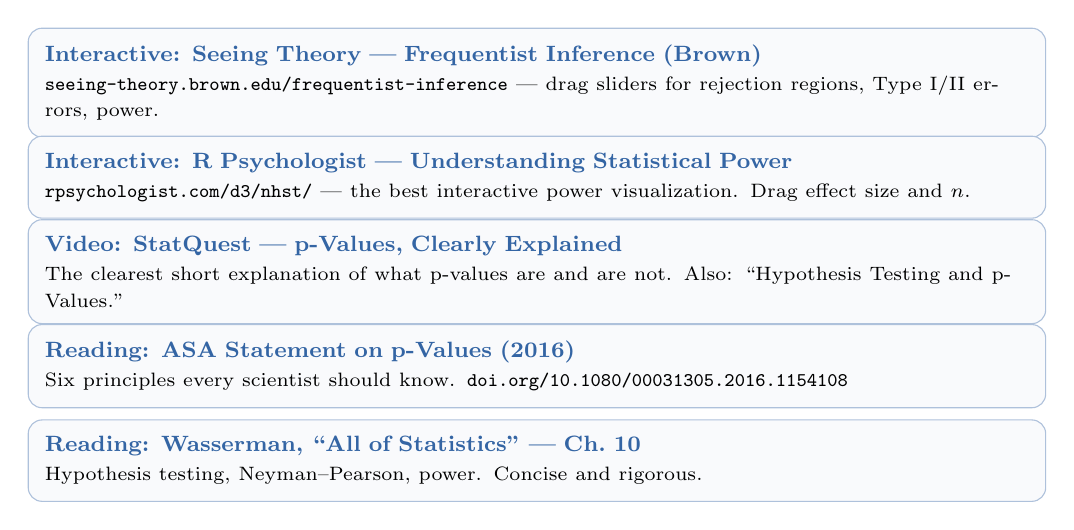
\begin{tikzpicture}[
  rbox/.style={draw=popblue!40, fill=popblue!3, rounded corners=5pt, text width=12.5cm, align=left, inner sep=6pt, font=\footnotesize}
]
  \node[rbox] at (0, 2.4) {
    \textbf{\textcolor{popblue}{Interactive: Seeing Theory --- Frequentist Inference (Brown)}}\\[1pt]
    \scriptsize\texttt{seeing-theory.brown.edu/frequentist-inference} --- drag sliders for rejection regions, Type I/II errors, power.
  };
  \node[rbox] at (0, 1.2) {
    \textbf{\textcolor{popblue}{Interactive: R Psychologist --- Understanding Statistical Power}}\\[1pt]
    \scriptsize\texttt{rpsychologist.com/d3/nhst/} --- the best interactive power visualization. Drag effect size and $n$.
  };
  \node[rbox] at (0, 0.0) {
    \textbf{\textcolor{popblue}{Video: StatQuest --- p-Values, Clearly Explained}}\\[1pt]
    \scriptsize The clearest short explanation of what p-values are and are not. Also: ``Hypothesis Testing and p-Values.''
  };
  \node[rbox] at (0, -1.2) {
    \textbf{\textcolor{popblue}{Reading: ASA Statement on p-Values (2016)}}\\[1pt]
    \scriptsize Six principles every scientist should know. \texttt{doi.org/10.1080/00031305.2016.1154108}
  };
  \node[rbox] at (0, -2.4) {
    \textbf{\textcolor{popblue}{Reading: Wasserman, ``All of Statistics'' --- Ch.\ 10}}\\[1pt]
    \scriptsize Hypothesis testing, Neyman--Pearson, power. Concise and rigorous.
  };
\end{tikzpicture}
\end{center}
\end{frame}

\begin{frame}
\begin{center}
  {\Huge\bfseries\textcolor{popblue}{Questions?}}

  \vspace{1cm}

  {\large Next: Lecture~10 --- $t$-tests, chi-squared, likelihood ratio tests}
\end{center}
\end{frame}

\end{document}
